Le contrôleur exécute potentiellement des applications fournies par des tiers. Si un utilisateur  importe une application malveillante sur le contrôleur, cela peut avoir des répercussions sur tout le réseau.
En appliquant la méthode STRIDE à l'interface nord, on trouve 5 menaces :

\begin{itemize}

\item Altération (T) : possibilité de modifier le flux de données des applications en se plaçant sur le chemin du contrôleur (man in the middle). Cette partie est rapide à étudier puisque là encore, TLS, si il est correctement utilisé, permet d’éviter toute modification du flux d'information.

\item Répudiation (R) : possibilité pour une application de nier certaines actions dont elle est l'origine.

\item Divulgation d'informations (I) : possibilité d’obtenir des informations sur d'autres applications, sur l'état général du contrôleur, ...

\item Déni de service (D) : possibilité d'action néfaste sur le contrôleur (modification de la topologie, dégradation du débit offert par le contrôleur, ...).

\item Escalade de privilège (E) : possibilité de modifier le comportement de certaines applications avec des droits non adaptés.

\end{itemize}

Dans la suite, on testera T, D, I et E. Ici encore cela sera fait par rapport à ONOS, ce qui se justifie d'avantage (aucun standard n'existant au niveau de l'interface nord, celle-ci peut varier selon le contrôleur). De plus, ONOS propose un mécanisme de sécurité intéressant à étudier qui est le Security Mode, mis en place depuis la version Drake (1.3) du contrôleur.

\begin{figure}[h]
  	\centering
  	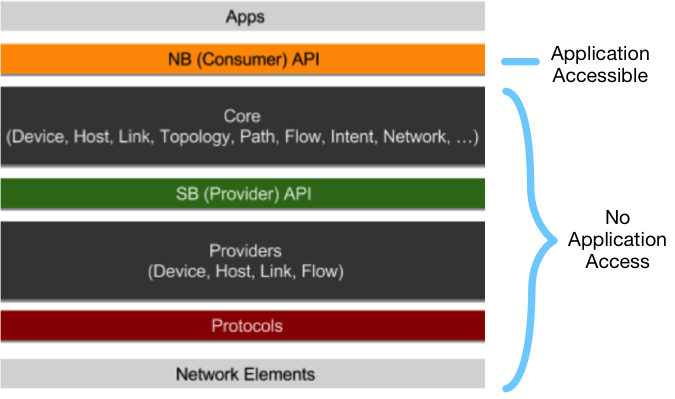
\includegraphics[width=0.6\textwidth]{secure_mode.png}
  	\caption{Security mode activé : accès aux fonctions critiques restreint lors de l'utilisation de l'API par certaines applications}
\end{figure}

Ce module, qui continue d'être amélioré, ajoute la possibilité de définir des permissions fines (ce qui se traduit par le droit d'utiliser ou non certaines fonctions de l'API) pour les applications, et sera légèrement détaillé plus tard. Les attaques qui constitueront cette partie seront donc moins génériques que les attaques menées au niveau de l'interface sud.
